\documentclass[12pt,a4paper,twoside,titlepage]{memoir}
\usepackage[utf8]{inputenc}
\usepackage{amsmath}
\usepackage{amsfonts}
\usepackage{amssymb}
\usepackage{graphicx}
\usepackage{color}
\usepackage{tabularx}
\usepackage{cite}
\usepackage{float}
\usepackage{soul}
\usepackage{tcolorbox}
\usepackage[marginparsep=-1.8cm]{geometry}
\chapterstyle{section}
%\setcounter{chapter}{+1}
%\counterwithout{section}{chapter}
\newcommand{\todo}{\textcolor{red}{\textbf{TODO}}}

\newcommand{\markIt}{\strut\vadjust{\domark}}
\newcommand{\domark}{%
	\vbox to 1pt{
		\kern-\dp\strutbox
		\smash{\llap{***\kern1em}}
		\vss
	}
}

%\title{Investigating Visual Perspectives on Guidance Visualisations for Motor Learning}
%\date{December 2019}
%\author{Stefan Paul Feyer}
%\author{Supervisor Maximilian Dürr}

\title{Investigating Visual Perspectives on Guidance Visualisations for Motor Learning}
\author{Stefan Paul Feyer\\
	\textit{HCI Group, University of Konstanz}
	\and
	Maximilian Dürr\\
	\textit{Supervisor}
	\and
	Prof. Dr. Harald Reiterer\\
	\textit{Examiner}
}
\date{Seminar to the Master's Project \\December 2019}


\begin{document}
	\maketitle
	\thispagestyle{empty}
	%\reversemarginpar%maring left
	\frontmatter
	%\section*{Abstract}
\chapter*{Abstract}

	sfgsdfgsdgsdfgsdfgdsfgdsfgsdfg
\begin{itemize}
	\item Overall aim of the Seminar thesis: how to investigate the influence of perspectives on virtual avatars in MR for motor learning
	\item therefore analysis of motor learning, related work, research questions
	\item propose study setting
\end{itemize}

	\begin{KeepFromToc}
		\tableofcontents
	\end{KeepFromToc}
	\listoffigures
	\listoftables
	\mainmatter
	\chapter{Introduction}

\section{Motivation}
%heranführung zum thema, erklären warum das wichtig ist.
In recent years, Mixed Reality (MR) devices became affordable \footnote{\hyperlink{https://www.vive.com/}{vive.com}, \hyperlink{https://www.oculus.com/}{oculus.com}accessed: 3.12.2019}, portable \footnote{\hyperlink{https://arvr.google.com/daydream/}{arvr.google.com/daydream} accessed: 3.12.2019} and usable in many conditions. Not only academic researchers are interested in this technology, commercial companies also found MR devices helpful to explore new possibilities to use it profitable. With this development, learning and training in MR became possible for many cases, too. EON \footnote{\hyperlink{https://www.eonreality.com/}{https://www.eonreality.com/} accessed: 14.12.2018} for example calls themself "the world leader in Virtual Reality based knowledge transfer for industry, education, and edutainment". They develop MR programs for several platforms, eg. with the aim to guide workers, reducing mistakes and thus reducing costs. These programs address a lot of use cases in the field of education, energy, health \& medical, manufacturing \& industrial, defence \& security and aerospace. Tasks include eg. ground crew training for a Boeing 777, augmented reality (AR) assembly training, exploring or anatomy simulation to mention only a few, compare \ref{fig:eonreality}.
\begin{figure}
	\centering
	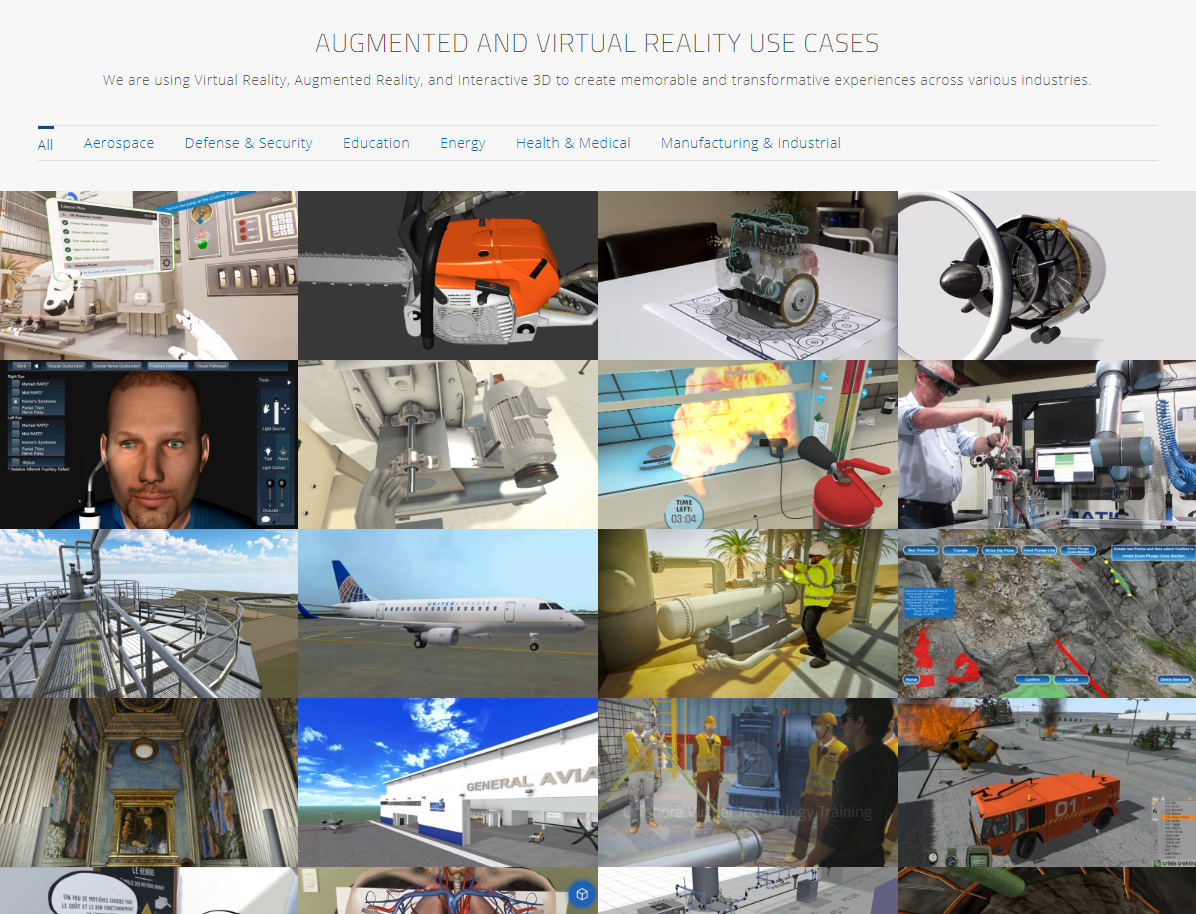
\includegraphics[width=1.0\textwidth]{img/eonreality.PNG}
	\caption{Usecases by EONReality on their AVR plattform.  \hyperlink{https://www.eonreality.com/use-cases/}{eonreality.com/use-cases/} accessed 30.07.2019}
	\label{fig:eonreality}
\end{figure}
Microsoft also stepps into this topic with partners, developing tools for apprentice, maintenance, or remote training. Eg. The Smart Glass experience Lab\footnote{\hyperlink{https://www.fit.fraunhofer.de/de/fb/cscw/smart-glasses-experience-lab.html}{fit.fraunhofer.de/de/fb/cscw/smart-glasses-experience-lab.html} accessed: 18.11.2019} of the Fraunhofer Institute use the MS Hololens \footnote{\hyperlink{https://www.microsoft.com/en-us/hololens}{microsoft.com/en-us/hololens} accessed: 3.12.2019} for remote maintenance, compare figure \ref{fig:fraunhofer}.
\begin{figure}
	\centering
	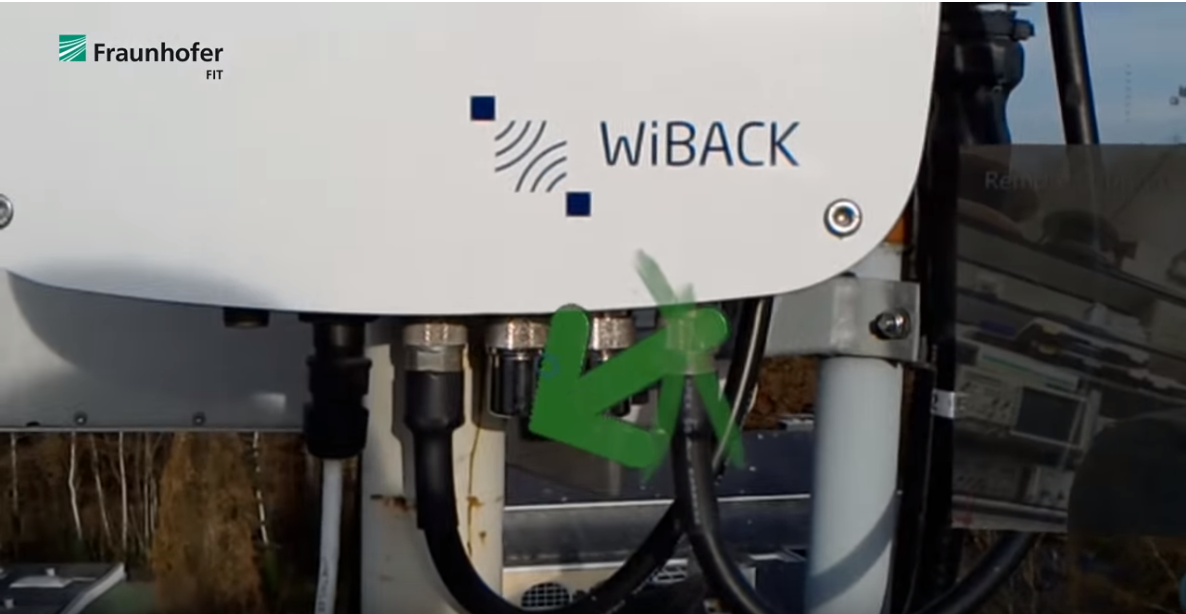
\includegraphics[width=1.0\textwidth]{img/fraunhofer.PNG}
	\caption{Remote maintenance with Hololens by Smart Glass Experience Lab. The on site worker wears a Hololens, while the remote trainer draws green hints to resolve a miswiring, taken from \hyperlink{https://www.youtube.com/watch?v=1QFMPo5k6p0}{https://www.youtube.com/watch?v=1QFMPo5k6p0}, accessed (30.07.2019)}
	\label{fig:fraunhofer}
\end{figure}\\
For developing MR learning and training environments, research put effort in developing how-to's and guidelines to ensure proper systems e.g. \cite{LaViola2017}. However - as we will see in Chapter 3 - there is a research gap about the visual perspective in these systems. For example, a student wants to learn a movement from a teacher. In the real world, the teacher stands in front of the student preforming the movement and the student tries to mimic it. This perspective is called exocentric or 3rd person. In contrast, in MR we have the possibility to change this perspective what we cannot do in the real world. A student can "step into" the teachers virtual body and see the instruction from the 1st person view of the teacher, also called egocentric view. Changing the perspective could have influence on the learning. This rises the following question: Does the perspective has influence on learning in MR environments? 
This seminar thesis is the first out of three parts, followed by a Masters Project and a Masters thesis. The overall aim of this work is to answer the following main research question:
\begin{itemize}
	\item[MRQ] Does the visual perspective on a virtual guidance visualisation have an influence on motor learning in MR environments.
	
\end{itemize}
The outcome in this work is a study design that will be able to address the research questions. In the Masters project the proposed study setting will be implemented, to be able to conduct the study and collecting the necessary data to answer the question. The Masters thesis itself will take the generated data to answer the research question.


\section{Outline}
For a proper study design many aspects must be taken into consideration. The main aspects this thesis will discuss are defined in the following, while further aspects like algorithms are discussed in the masters project. In Chapter 2 this work sets the scope and provides theoretical foundations. in Chapter 3 the parameters for the study design are discussed by means of related work. With the scope and parameters set, Chapter 4 proposes a study design which serves as base for the Masters project. In the end, an outlook on further work on the Masters thesis is given. Compare figure \ref{fig:overallProcess}.
\begin{figure}
	\centering
	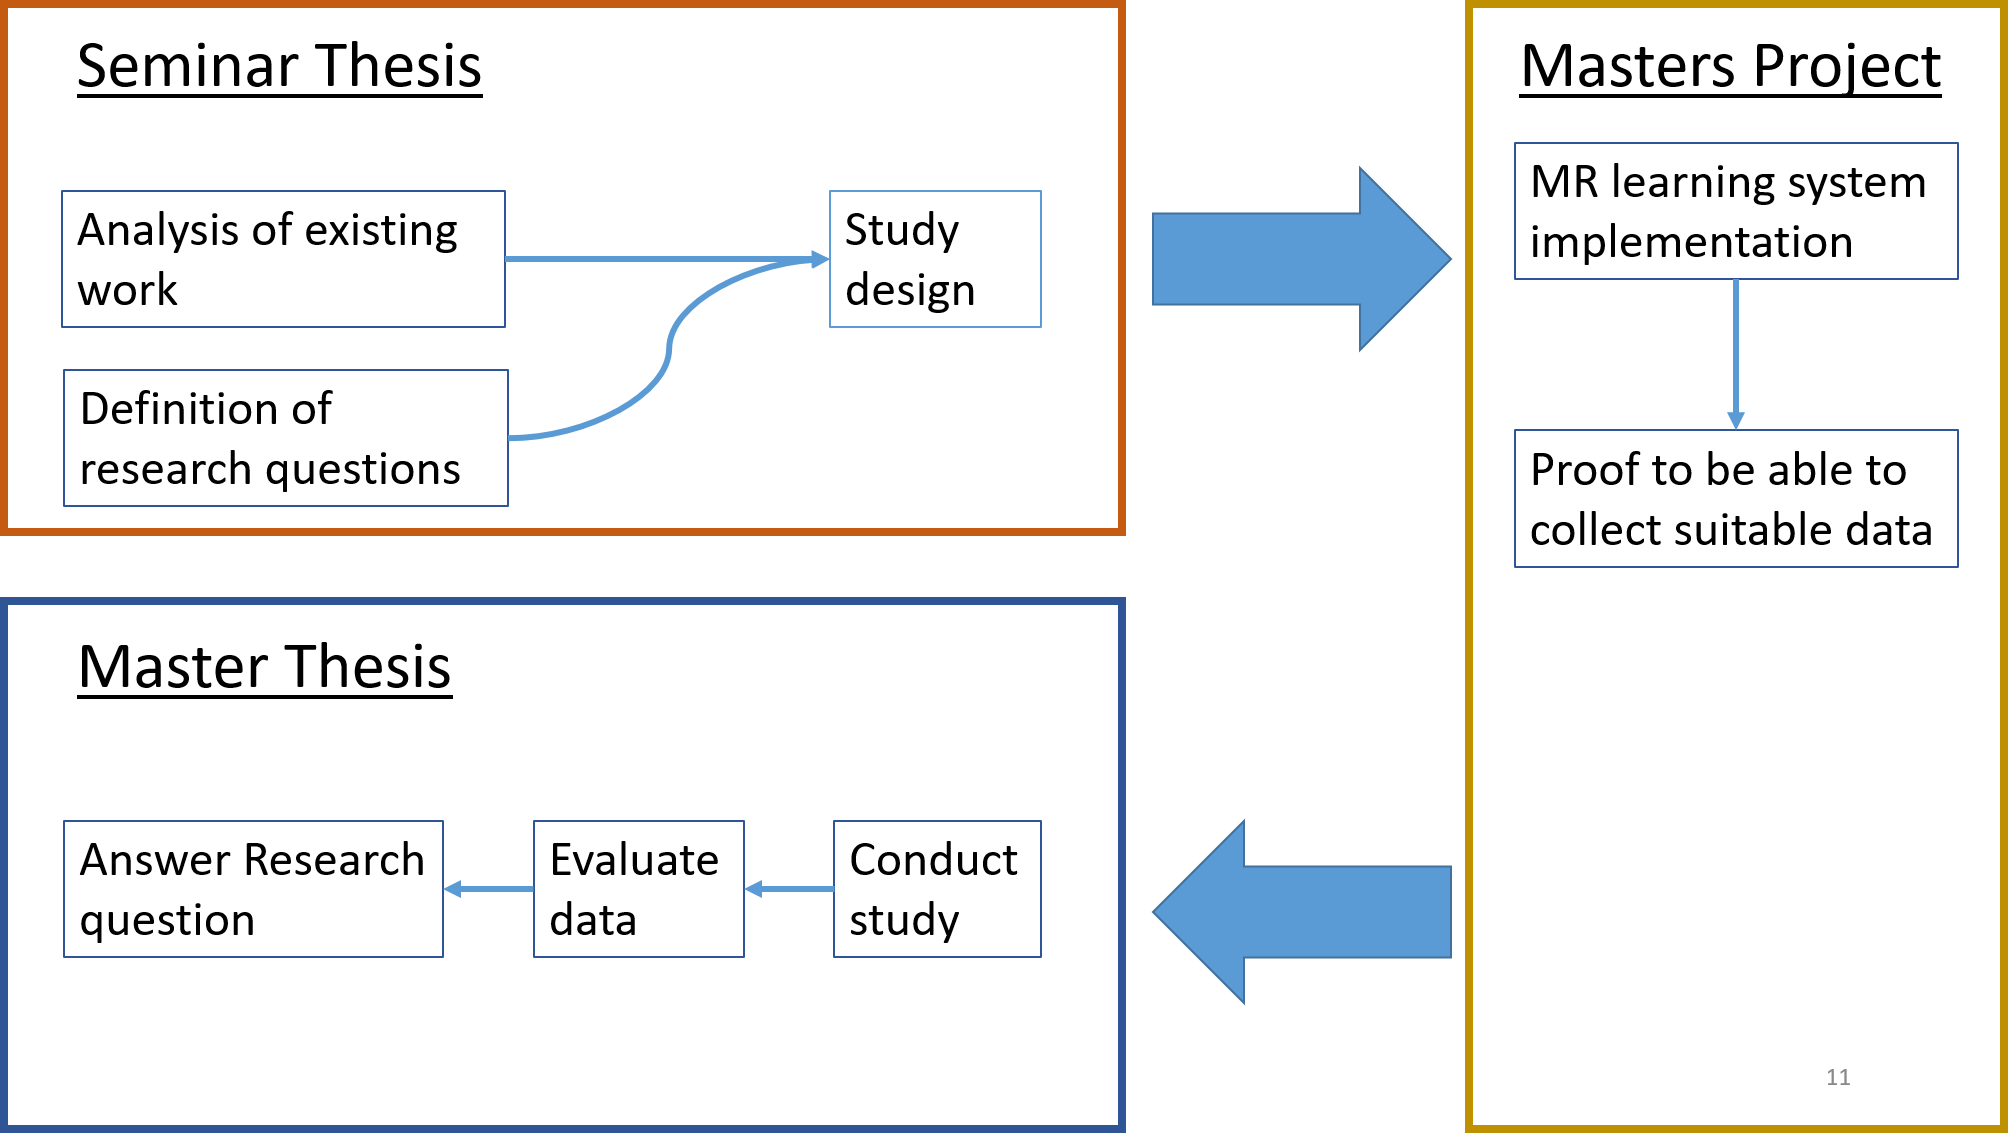
\includegraphics[width=1.0\textwidth]{img/overallProcess.png}
	\caption{Overall process of the masters thesis.}
	\label{fig:overallProcess}
\end{figure}\\

%Each of these aspects must be chosen wisely. In order to do so this seminar thesis will systematically go through every one of them. Chapter 3 sets the scope of the study and provides general knowledge about the domain. The following chapter 4 analyses the work of researchers and their systems, to find suitable components for the scope that has been set in chapter 4. Here, the remaining aspects are analysed from a more practical view and it is investigated how researchers decided about the aspects and why. Whenever a decision is made to be used in the proposed study design, a symbol on the side of the text can be found \markA. After all aspects are clear and reasoned, a study design is proposed in chapter 5. 

%first the theoretical background will be taken into consideration. It is mandatory to know how humans learn, classify, quantify and measure movements. In addition, recent MR hardware and tracking technology is investigated, a classification of perspectives is given and also a insight on MR itself. In this chapter we also set the res
%This seminar thesis will have a look at the grounding principles to define a system that lead to the guidelines in question. Therefore we first step into the theoretical background in the next chapter. We will investigate how people achieve motor skills, how to quantify and measure movements, what hardware techniques are suitable, perspectives and mixed reality. In the following chapter we analyse how other researchers used the theory to gain insights in Motor learing in VR. In the end we propose a study setting to that can be used to investigate on this topic.
%After this introduction, the scope of this thesis is given, where it is explained to what extend motor learning, MR, perspectives and other factors are considered. The following related work part will give an overview about other MR learning systems and also work about perspectives on avatars. From this work the measures, dependent and independent variables and tasks are derived. Taking the related work into consideration a study design is proposed in outlook section.
	\chapter{Theory and Scope}

Motor learning in MR builds on many aspects, eg. suitable technology for MR representations and what perspectives to use. Furthermore, human motor learning must be suitably transfered in the digital world. And eventually, we need to match movements and measure the error correctly to derive adequate from the performance of a learner. In this chapter we take a look into these topics. If not other indicated, adopted from the book Motor Learning and Skills\cite{Schmidt2011}.

\section{Visual Perspectives}
\markAoneIndependent
Wang and Milgram \cite{Wang2001} describe the perspectives on the centricity continuum see figure \ref{fig:ego-exo-cont}. On the most left hand side of the continuum the egocentric perspective is located. Egocentric means that the anchor of the viewport camera is located inside the object to control - for simplicity, this object in question is referred as avatar. On the left hand side the exocentric perspective is located. This viewport camera is a fixed camera in the scene not to be controllable. The exocentric perspective gives the user the possibility to examine the scene from a bird's-eye view. The movement or angle of the avatar has no influence on the cameras position or angle. So the main difference is the so called tether distance and the degree of freedom of the camera. Milgarm and Wang investigated on tethered cameras and define it as the distance between the avatar and the camera which is following the avatar. This describes the middle part of the continuum. Zero-distance camera describes the egocentric perspective. The longer the tether distance the more the perspective is located on the right of the scale to the exocentric perspective. They also distinguish between dynamic and rigid tethering relation ships. A dynamic tethered camera is controlled by the user in all six dofs (\todo) while a rigid stands like a pole and can only be controlled in 3 dofs. Rigid tethered cameras are common in modern 3rd person computer games.
\begin{figure}
	\centering
	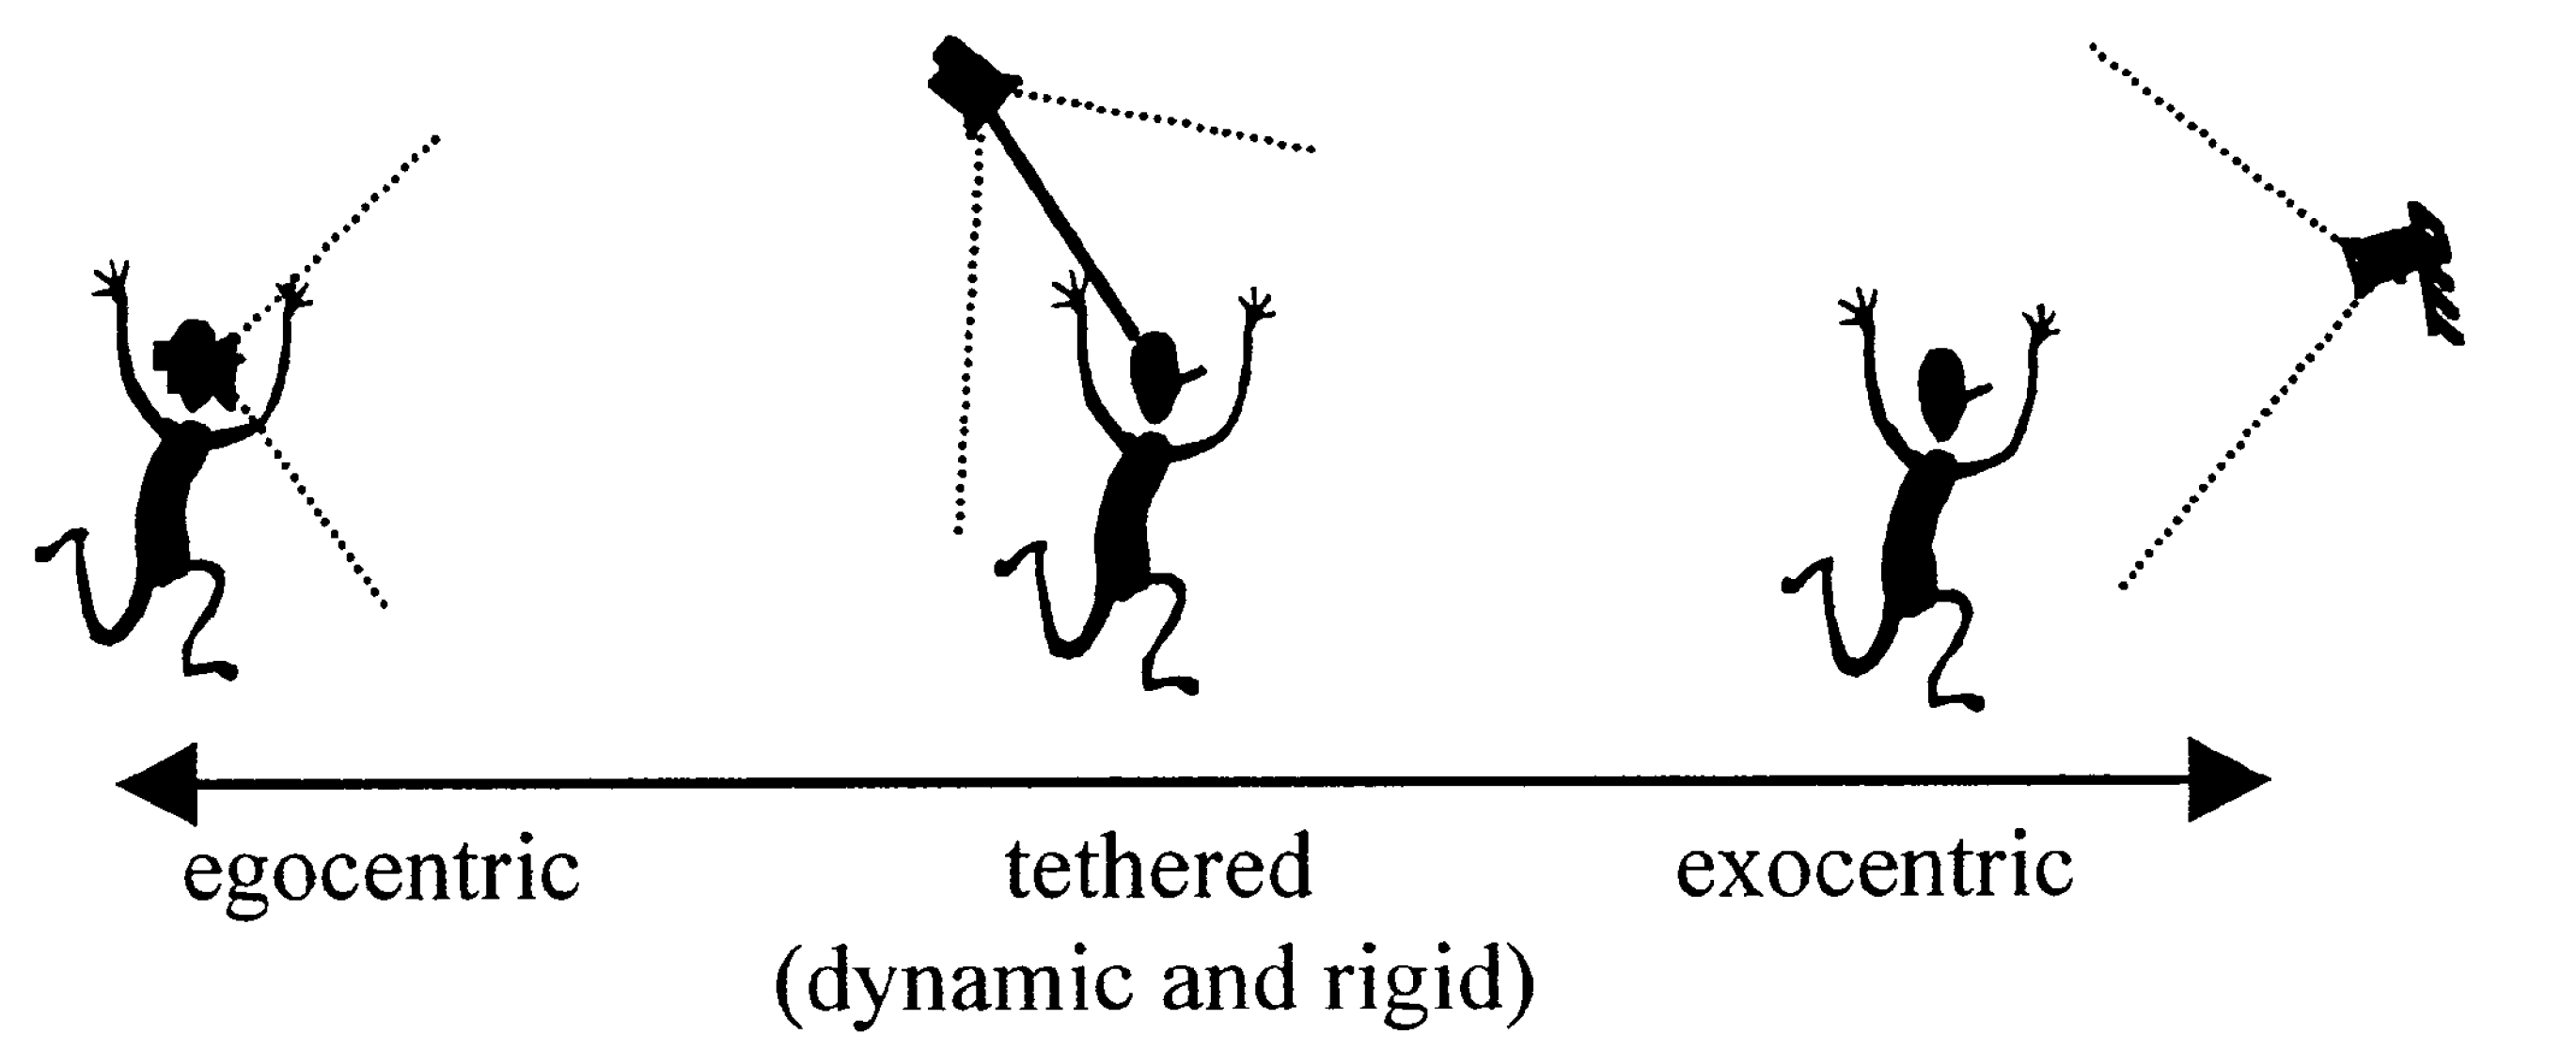
\includegraphics[width=1.0\textwidth]{img/ego_exo_continuum_bigger.PNG}
	\caption{Centricity continuum by Wang and Milgram 2001 \cite{Wang2001}}
	\label{fig:ego-exo-cont}
\end{figure}
\markAsixPerspective

\subsection{Degree of realism of teacher avatar}
first some paper collection about how the virtual avatar looked like, and then decide for what rebeccas work proposes. its a lot about related work, so maybe this should go in the next chapter. what would be more work. \markAonefourRealism

\subsection{Feedback and instruction behaviour}
feedback \todo can be given verbally, in MR visually ... example 1,2 and 3, but in the end: we do not want to evaluate feedback so there will be none in the study \markAonefiveFeedback. In addition, for high validity instructions must be the same, so a pre recorded instructions necessary \markAelevenBehav partly answered, but lets look in next chapter about continuity in instruction.

\section{Motor Learning}

\subsection{Learning movements}
\textbf{In the real world} Motor learning takes place by instruction, trying, imitation or a combination of two or all three. A learner can observe another person and imitate the movement, try to accomplish a task by themself or can follow instructions. Instructions can be written, visual or verbal. Written instructions are not bound to words solely, eg. Rudolf van Laban developed a dace notation system, compare section "quantify movements" \ref{quantifymovements} and figure \ref{fig:laban}. Visual or verbal instruction include a trainer, teaching the student movements. In this case verbal and physical feedback also plays a role in the learning process. The process of motor learning is divided in three parts. Once a student starts learning using what ever technique, it starts in the \textit{cognitive} state. In this stage the students tries to figure out what is to be done to achieve the task. For this high cognitive activity is required, strategies are evaluated. The performance gains dramatically and is larger than in any other stage, but also inconsistent. The use of instructions and other training techniques are most effective. The next stage is the \textit{fixation}. It begins when the student had determined the most effective way of doing the task. Performance increases more gradually but becomes more consistent. In the last \textit{autonomous} stage, the performer gains proficiency and other tasks are less likely to interfere. Since the use of training techniques and the high performance gain in the \textit{cognitive} state, tasks in this stage are best suited for the study. This will be considered in the next chapter, too.\\
\textbf{In the digital world} most of this remains like it is in the real world. But with computational power new learning techniques can be used to teach motor learning. Instructions can be given visually by a teacher without the teacher being physically in the room, eg. by video instructions or virtual avatars. Also remote instructions become more practical eg. in video conferences. 

\subsection{Movement classification}
For a simplified discussion a classification of movements is provided in the following. There are two important classification schemes. The first one is based on the particular movements performed and are divided into \textit{discrete}, \textit{continuous} and \textit{serial movements}. The second one is based on perceptual attributes of the task and are divided into \textit{open} and \textit{closed skills}. Both classification representing a continuum.

\subsubsection{Discrete, Continuous and Serial Movements}
\begin{figure}
	\centering
	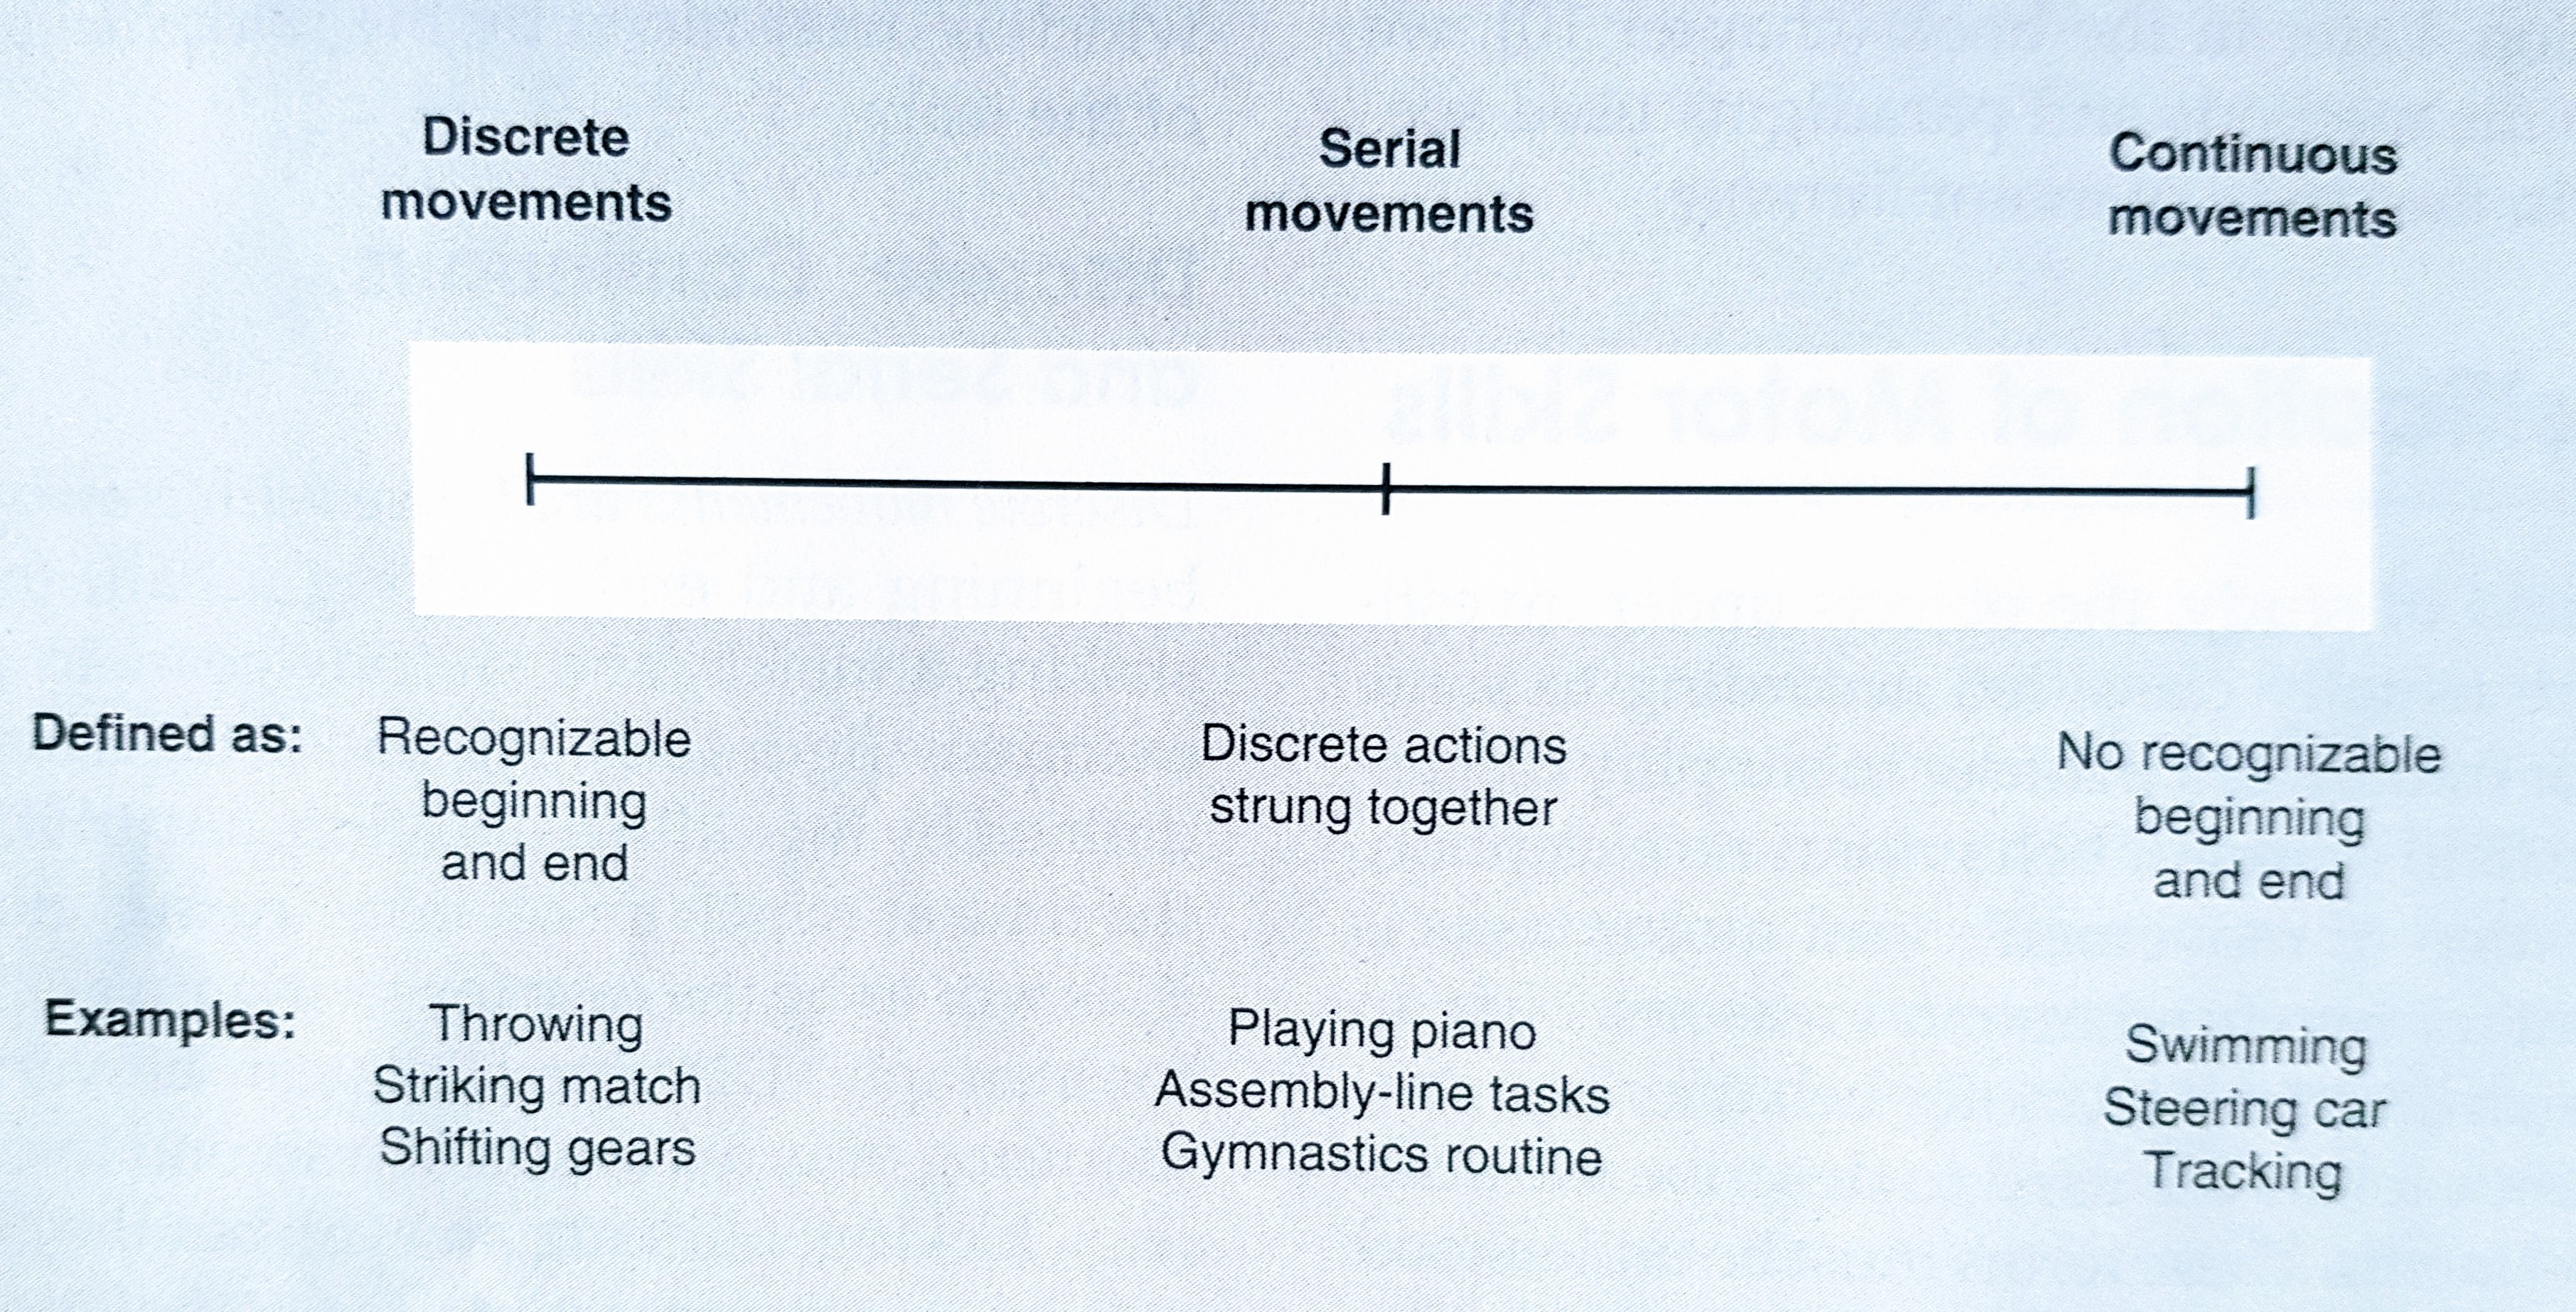
\includegraphics[width=1.0\textwidth]{img/movements_cont.jpg}
	\caption{Continuum of movements buch \cite{Schmidt2011}}
	\label{fig:movements_cont}
\end{figure}
\textit{\textbf{Discrete movements}} are located on the one end of the continuum. These are movements with a recognisable beginning and end. The end of a discrete movement is defined by the task itself and can be very rapid like blinking or longer like making the signing. Examples are kicking a ball, shifting gears in a car or striking a match\\
\textit{\textbf{Continuous movements}} are located on the other end of the continuum. These movements don't have a recognisable start and end, with behaviour continuing till the movement arbitrarily stopped. Continuous tasks tend to be longer than discrete tasks. Examples are swimming, running or steering a car.\\
\textit{\textbf{Serial movements}} are located in the middle part of the continuum. Following the nature of a continuum these movements are neither discrete nor continuous. They can consist of smaller movements tied together. Furthermore, discrete movements can be rather long but are not stopped arbitrarily. Serial tasks can be seen as many discrete tasks strung together and the order (and sometimes timing) is important. Examples are starting a car or preparing and lighting a wood fireplace.\\
The nature of \textit{Continuous movements} having no recognizable beginning and end makes it hard to describe a distinctive task for a study design while \textit{discrete movements} are to short for a proper task, \textit{serial movements} are choose for the study task \markAthreeMovClass.

\subsubsection{Open and Closed Skills}
\textit{\textbf{Open skills:}} The environment is constantly, unpredictably changing, so the performer cannot plan his activity effectively in advance. Own movements depend on the environment. For example, if a ice hockey player shoots a shot in ice hockey, his own movement is dependent on the movement of the keeper. Another example is  driving on a free way. The driver needs to adjust his own driving dependent on the behaviour of the other cars. Success in open skills is largely determined by the extend to which a individual can adapt the planned motor behaviour to the changing environment.\\
\textit{\textbf{Closed skills:}} The environment is predictable, mainly because it is stable. This means that the performer can plan his activity in advance. Examples are bowling, archery or singing. To evaluate only the motor learning and not environmental influences the study is conducted in a controlled environment in a laboratory. Thus only \textit{closed skills} are taken into consideration \markAfourSkills.

\begin{figure}
	\centering
	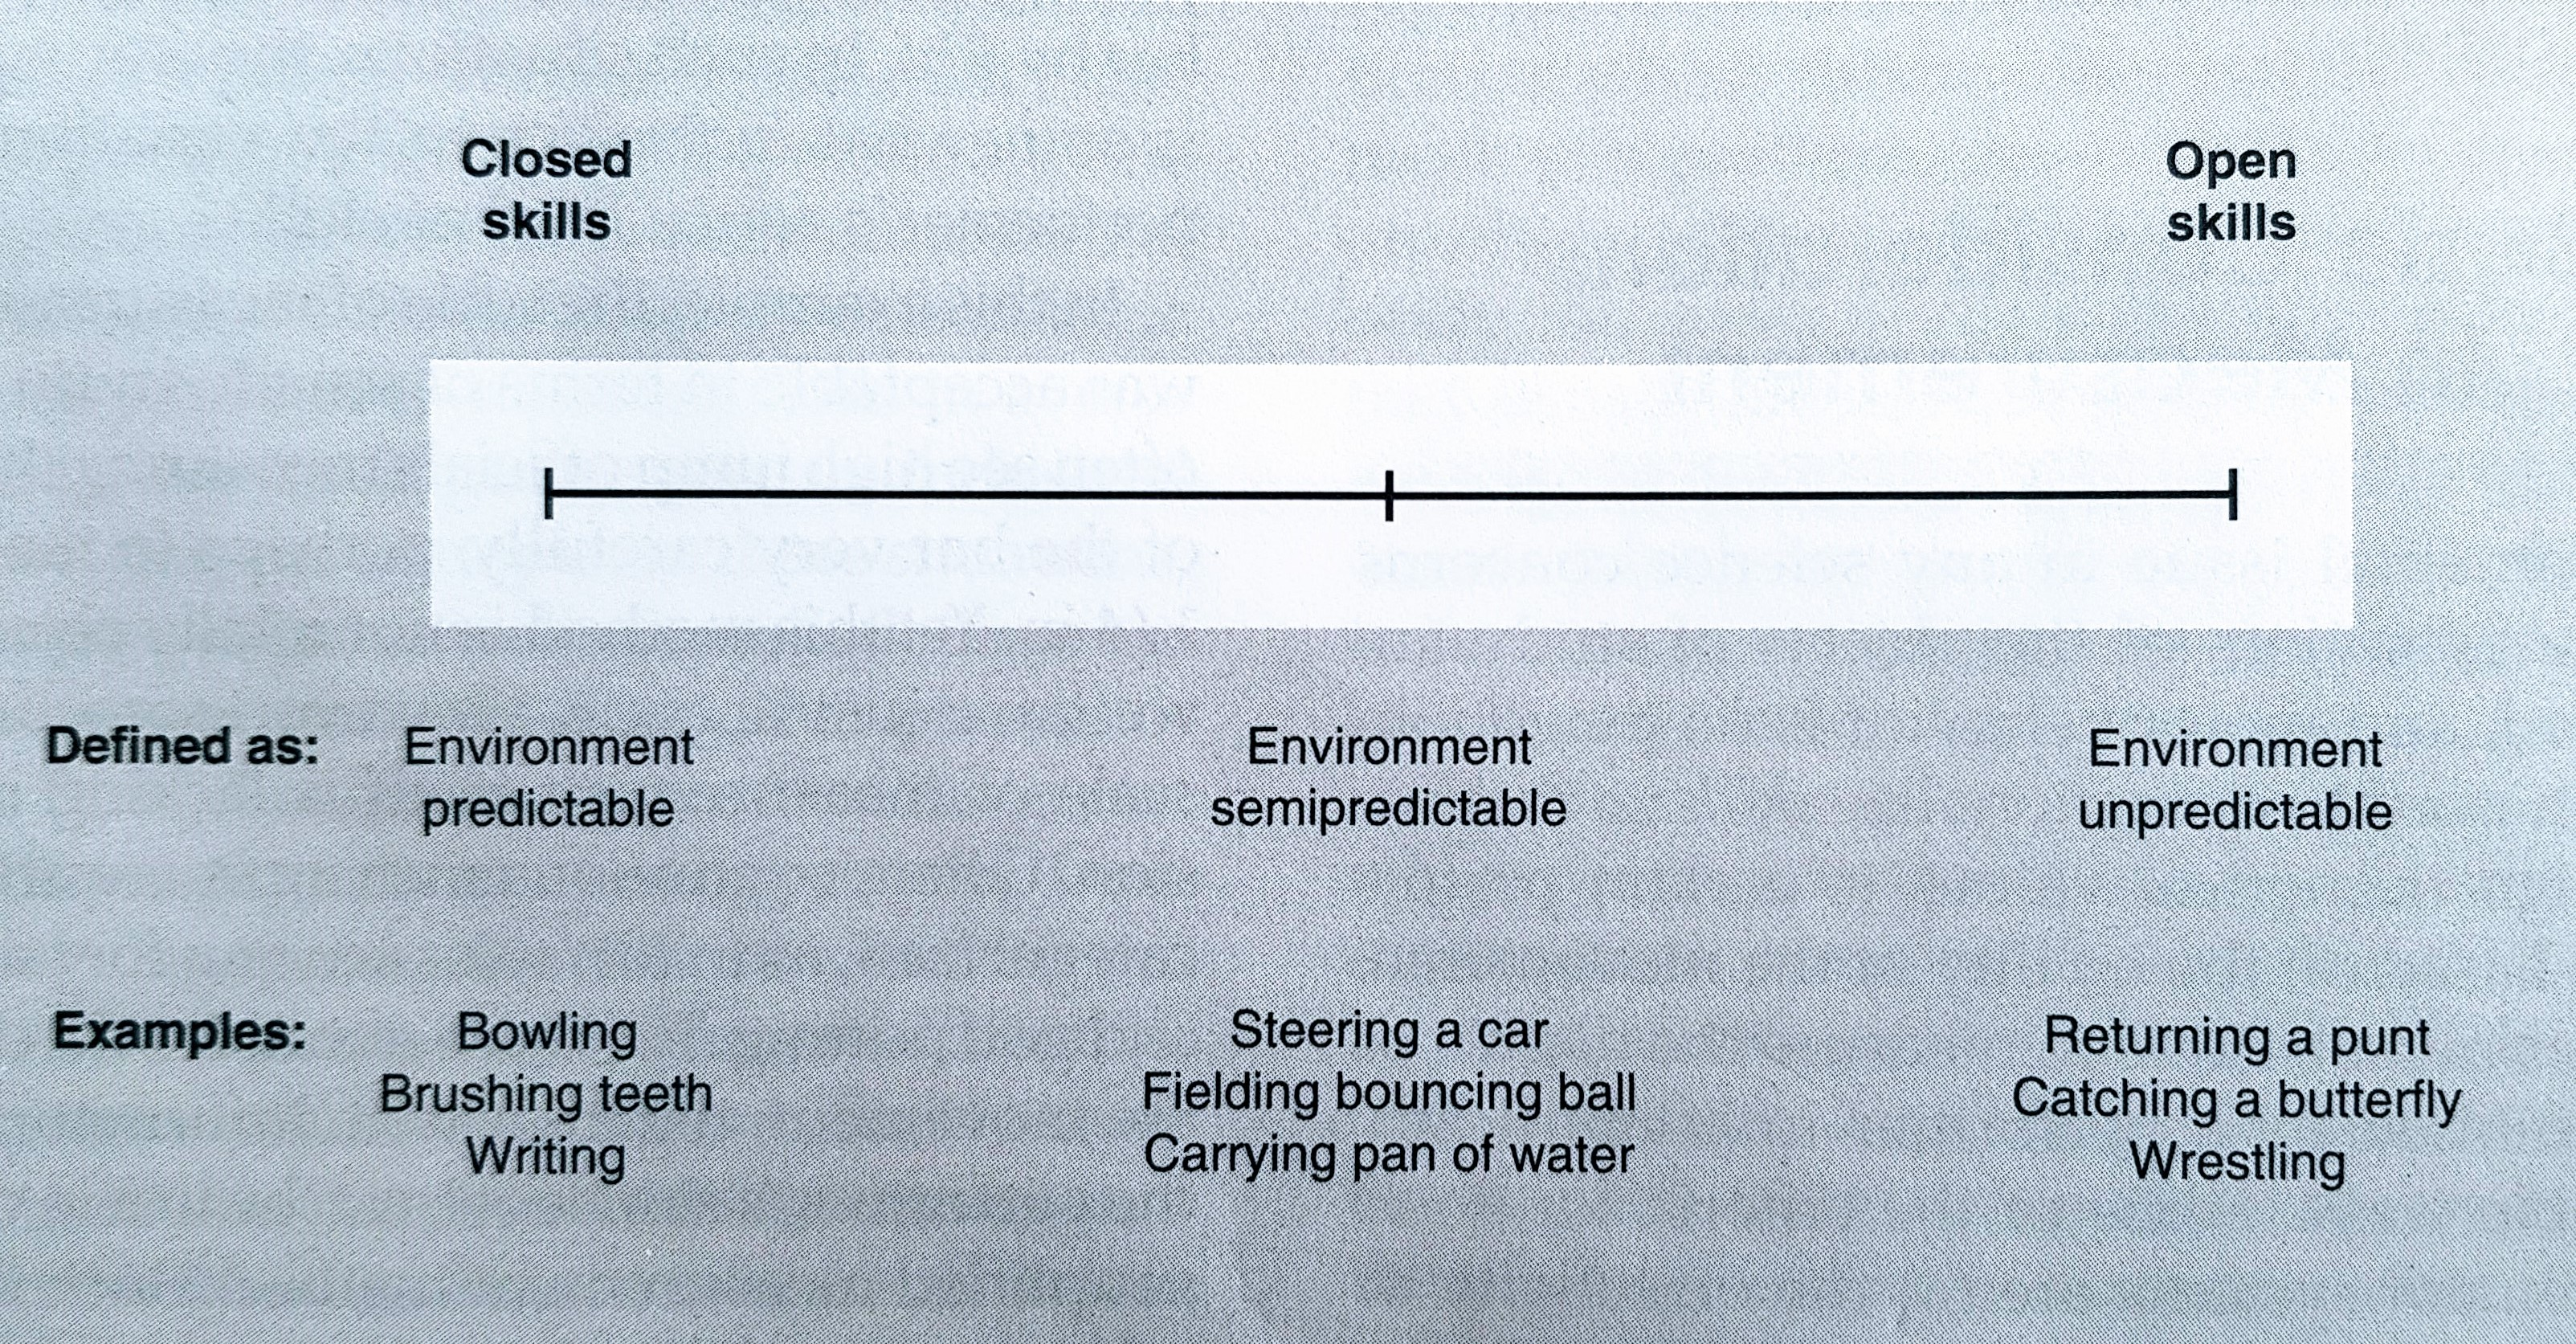
\includegraphics[width=1.0\textwidth]{img/skills_cont.jpg}
	\caption{Continuum of skills \cite{Schmidt2011} \todo seite}
	\label{fig:skills_cont}
\end{figure}
%since open skills  seems to require rapid adaptions to a changing environment and closed skills require a very stable performances in a predictable environment questions are raised about the method of training, do different individuals perform better in in one of these skill classes. to overcome these question the focus of this seminar is on discrete movement tasks and closed skills. $->$ see study \todo + citations

%gespiegelte, ungespiegelt, synchron, asynchron -> max fragen

\subsection{Quantify movements \todo in measures} \label{quantifymovements}
%Wie können bewegungen überhaupt quantifiziert werden
\begin{figure}
	\centering
	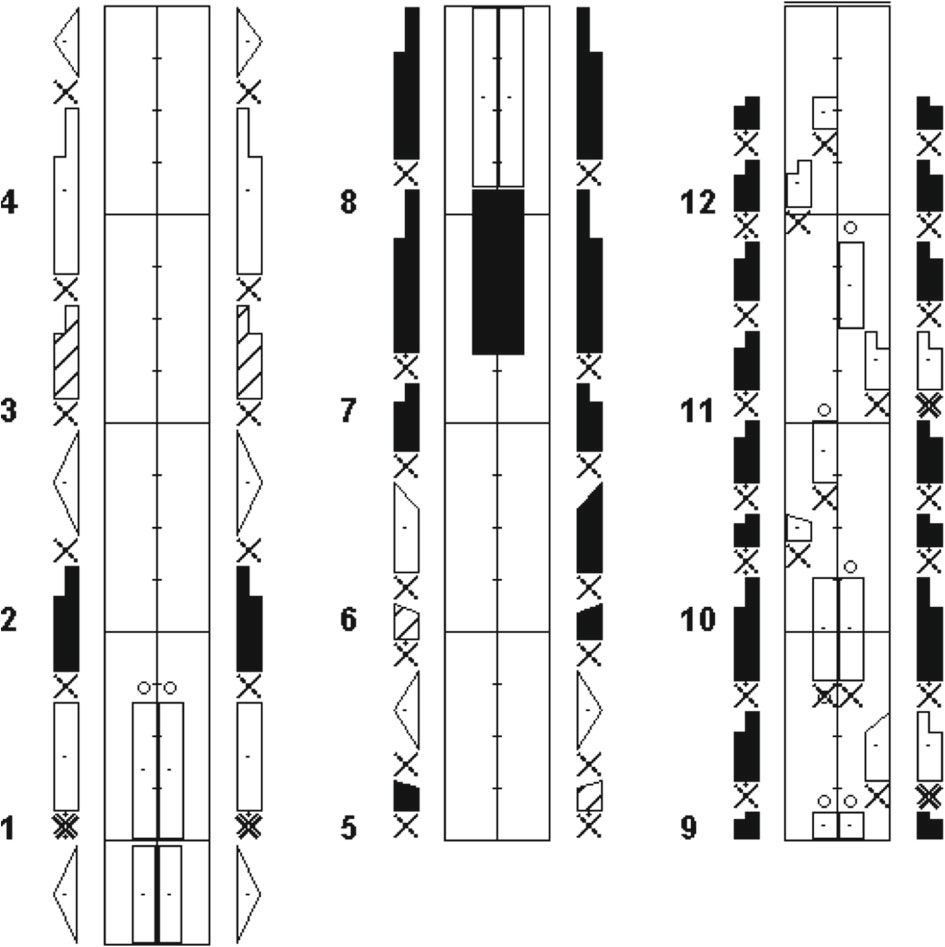
\includegraphics[width=0.5\textwidth]{img/laban.png}
	\caption{Laban notation. Generated through automatic movement interpretation by Choensawat \cite{Choensawat2015}}
	\label{fig:laban}
\end{figure}
Judging motions and matching them to a given motion is not a trivial task. Since eg. dancing is a pure physical task, movements must be recognised, digitalised and judged. One approach is to use a analog descriptions for dancing and translate them in the digital world. Choensawat \cite{Choensawat2015} began with Rudolph von Laban - a professional dancer. Von Laban developed a broadly used dance notation. His work lead to the \textit{Laban Movement Analysis} with which human movements could be quantized.\footnote{Brockhaus, Rudolf Laban. http://www.brockhaus.de/ecs/enzy/article/laban-rudolf (accessed 2018-10-25)} There are four main components to systematically describe movements in the \textit{Laban Movement Analysis}: body, effort, shape and space. Each component can describe movements independently or combined. Hachimura et al. \cite{Hachimura2005} used the methodology  of \textit{Laban Movement Analysis} and adopted it to for digital movements.\\
Yoshimura et al. \cite{Yoshimura2005} followed a similar approach from another dance movement description theory called \textit{furi}. \textit{Furi} is also described by four so called \textit{indices}: \textit{kamae}, \textit{jyu-shin}, \textit{koshi}, \textit{uchiwa}. Yoshimura at all could map these indices to concrete markers on the body of a performer.
%They showed that there was a significant difference between movements by an expert and a beginner.
Qian et al. \cite{GangQian2005} developed a gesture recognition system for performing arts. To match the motions ten body parts were defined: head, torso, upper arms, forearms, upper legs and lower legs. For each body part the Mahalanobis distance is calculated to an ideal point. The Mahalonobis distance describes the distance between point \textit{p} and distribution \textit{D}.\\
So the takeaway message is, there is a need to digitalise movement and then apply suitable algorithms to judge these movements. The algorithms will be discussed in the Masters project.

\begin{comment}
Kwon et al. \cite{Kwon2005} \todo 
\begin{itemize}
	\item K. Hachimura, K. Takashina, and M. Yoshimura, “Analysis and
	Evaluation of Dancing Movement Based on LMA,” Proc. IEEE Int’l
	Workshop Robots and Human Interactive Comm., pp. 294-299, 2005.
	\item M. Yoshimura, N. Mine, T. Kai, and L. Yoshimura, “Quantification	of Characteristic Features of Japanese Dance for Individuality Recognition,” Proc. IEEE Int’l Workshop Robot and Human Interactive Comm., pp. 193-199, Sept. 2001.
	\item G. Qian, F. Guo, T. Ingalls, L. Olson, J. James, and T. Rikakis, “A	Gesture-Driven Multimodal Interactive Dance System,” Proc. IEEE	Int’l Conf. Multimedia and Expo (ICME ’04), pp. 1579-1582, June	2004.
	\item D.Y. Kwon and M. Cross, “Combining Body Sensors and Visual
	Sensors for Motion Training,” Proc. ACM SIGCHI, pp. 94-101,	2005.
	\item vr dance trainer
\end{itemize}
\end{comment}


\subsection{Measuring movements}
%Welche messmethoden gibt es um bewegungen zu messen
In order to judge if a movement is performed correctly methods need to be applied to measure the error of a performed action. In literature, three main categories are listed: \textit{error of a single subject}, \textit{measures of time and speed} and \textit{measures of movement magnitude}. As chapter 3 will show, \textit{error of a single object} is most commonly used, the latter two are only discussed in short. 
\subsubsection{Measures of Error for a Single Subject}
Measures of error for a single subject represent the degree to which the target was not achieved. A target can be to perform an act at a particular time (time stamp), move with a certain force (amount of force) or hit a spatial target (a point in spatial volume). The attribute of the target serves as the variable in question, see braces behind the examples. The error itself describes the distance - in regard to the dimension - from the target. The following list gives an insight to the most important error measures.
\begin{itemize}
	\item \textbf{\textit{Constant Error}} describes the average error between the actual accuracy and the target. Means, in average the performer missed the target by CE.
	\begin{equation}
		CE=\frac{\sum_i(x_i-T)}{n}
	\end{equation}
	\label{eq:constanterror}
	with $x_i$: score, $n$: number of values, $T$: target value.
	\item \textbf{\textit{Variable Error}} measures the inconsistency in movements. The more consistent the movements, the smaller $VE$. $VE$ does not depend on whether or not the subject was close to the target.
	\begin{equation}
		VE=\sqrt{\frac{\sum(x_i-M)^2}{n}}	
	\end{equation}
	\item \textbf{\textit{Total Variability}} describes the total variability around a target. The combination of VE and CE represents the total amount of spread about the target. It is an overall measure how successful was the subject in achieving the target.
	\begin{equation}
		E=VE^2+CE^2=\sqrt{\frac{\sum(x_i-T)^2}{n}}
	\end{equation}
	with $x_i$: score, $n$: number of values, $T$: target value.
	\item \textbf{\textit{absolute error}} is a measure of the overall accuracy in performance.
	\begin{equation}
		AE=\frac{\sum|x_i-T|}{n}
	\end{equation}
	with $x_i$: score, $n$: number of values, $T$: target value.
	\item \textbf{\textit{Absolute Constant Error}} is the absolute value of $CE$. Because of negative and positive values can cancel each other out
	\begin{equation}
		ACE = |CE|
	\end{equation}
\end{itemize}


\subsubsection{Measures of Time and Speed}
Basic to this idea is, a performer who can accomplish more in a given amount of time or who can accomplish a given amount of behaviour in less time is  more skillful. Measures here are
$\frac{time}{unit}$ or $\frac{units}{time}$.\\
The two most common examples are \textit{reaction time} (RT) and \textit{movement time} (MT). Reaction time describes the amount of time between a stimuli and the regarding start of a movement. This time span is important for two reasons. On the on hand, RT has a high validity for real-life tasks, and, on the other hand, RT measures the time taken for mental events like stimulus processing or decisinón making.\\
\textit{Movement time} is the time interval between the end of the RT phase, though the start of the response, and the completion of the movement. The sum of RT and MT is called \textit{response time}.
%\underline{reaction time} (RT): can also be a performance measure. a measure of time from the arrival of a sudden and unanticipated signal to the beginning of the response. 

\subsubsection{Measures of Movement Magnitude}
To measure a skill, the produced magnitude of a behaviour can used. Eg. the distance a discus is thrown. A famous example is the "ski simulator". Rubber bands hold a plated centred between two poles. The magnitude in this case is the the dislocation of the board from the centre by using full body movements.

\section{Mixed Reality}
Mixed reality continuum \cite{Milgram1994} and something about when AR or VR is better. \ref{fig:MRcont} \todo \markAsevenMR

\begin{figure}
	\centering
	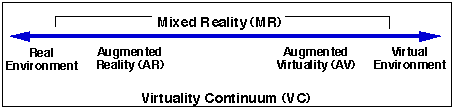
\includegraphics[width=1.0\textwidth]{img/milgram_continuum.png}
	\caption{Mixed reality continuum by Milgram et al. \cite{Milgram1994}}
	\label{fig:MRcont}
\end{figure}


\subsection{VR Technologies}
HMD,3D screens, tablets.... \todo or in project

\subsection{Motion Tracking Technologies}
External vs. internal tracking. Drift problem, accuracy... \todo or in project.



\section{Conclusion}
we dicided for A1 A2 ... will be used in study ... some aspects missing, lets have a look how other researchers choose there, what we do in the next chapter.
	\chapter{Related Work}
wie haben die anderen diese variablen untersucht
wie wurden die variablen untersucht $\rightarrow$ studiensetting
%----------------------------------------------------
\section{MR learning systems}


%----------------------------------------------------
\section{Ego/exo perspective work - if exists}

%----------------------------------------------------
\section{variables}
\begin{itemize}
	\item independent/dependent variables
	\item measures
	\item task: reuse or adapt existing task
\end{itemize}
%----------------------------------------------------
\subsection{Task}
\begin{itemize}
	\item Onebody: artificial postures not from but like: tai chi, matial arts
	\item VR Dance Trainer: dance movements
\end{itemize}
%----------------------------------------------------
\subsection{Measures}
\begin{itemize}
	\item onebody
	\item VR Dance trainer
\end{itemize}
%----------------------------------------------------
\section{Body parts included}
\begin{itemize}
	\item onebody
	\item vr dance trainer
	\item 
\end{itemize}
%----------------------------------------------------
\subsection{Independent and Dependent Variables}
\subsubsection{Dependent Variables}
\begin{itemize}
	\item VR
	\item bilateral movements
	\item Movement types: synchronous  / asynchronous 
\end{itemize}
\subsubsection{Independent Variables}
\begin{itemize}
	\item Body parts: upper body (UB), lower body (LB), full body (FB)
	\item Perspective: Ego, Exo, Ego/Exo combined
	\item Movement types: synchronous  / asynchronous 
\end{itemize}

write sth...

%----------------------------------------------------
\section{Conclusion}
\begin{itemize}
	\item task is xyz because of abc
	\item measures are xyz because of abc
	\item variables are...
\end{itemize}

	\chapter{Proposed Study Design}
Given the scope from chapter 2 and the parameters from chapter 3, this chapter proposes a study design. The study aims to produce data to answer the main research question from chapter 1:
\begin{itemize}
	\item[MRQ] Does the visual perspective on a virtual guidance visualisation have an influence on motor learning in MR environments.
\end{itemize}

\section{Setup}
For the study, a movement training system will be implemented. This movement training system will include a virtual reality HMD and motion-tracking technology. The student will be tracked with this motion capturing technology and with the resulting information, the student's avatar will be rendered as a high realism degree avatar. Likewise, the teacher avatar will be rendered, but not on the base of live motion tracking data. A professional Tai Chi trainer will be invited and a Tai Chi form will be recorded. This form will be split into 4 sub-forms. Furthermore, the teacher avatar will be scaled to the size of the student's avatar. To overcome the mirror issue, the student is allowed to move freely around the teachers' avatar. During the students' performance, the movement will be recorded and analysed in the aftermath with the discussed performance measure. 

\section{Procedure}
The study is conducted in a within-subject design with counterbalancing, which results in 32 participants, compare table~\ref{tbl:studySetting}. The student starts with the first visual perspective. The teacher appears and performs the movement, while the student is watching the performance. After the first demonstration, the student can train the motion simultaneously until the student is feeling confident, but caps after an amount of time which a pilot study has to reveal. After one of these cases, the final movement will be recorded, the student gets a short recovery rest. Then the next visual perspective starts. This process continues throughout all four conditions. Subsequent to the actual study, the post questionnaires will be answered. This questionnaire will contain questions about, perceived precision, ease to understand an preferred method.

\begin{table}
	\centering
	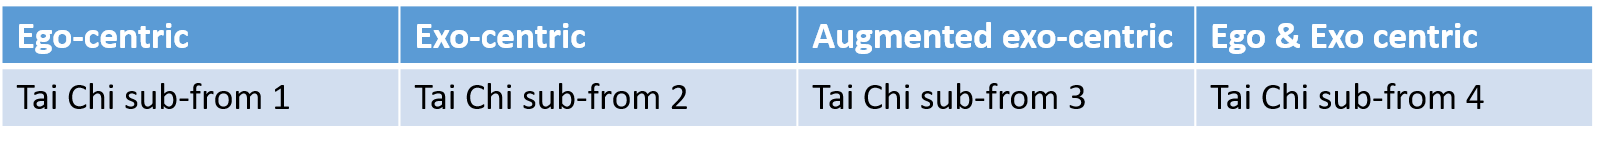
\includegraphics[width=1.0\textwidth]{img/studySetting.png}
	\caption{Study conduction schema.}
	\label{tbl:studySetting}
\end{table}

\section{Outlook}
The next step is to implement the study setup, but still, there are some parameters to refine on. This takes place in the master's project. In this part, the technology and algorithms will be in the main focus. For technology, VR HMDs will be compared and a decision will be made. Similar to motion tracking technologies. After this, algorithms for comparing two movements will be evaluated. When decisions are made, the implementation of the system will start. Eventually, a pilot testing session will take place followed by further refinements.
The milestones for the master's project are:
\begin{itemize}
	\item Hardware requirements: 17.1.2020
	\item Software Requirements: 24.1.2020
	\item Implementation Start: 27.1.2020
	\item Pilot Study: 2.3.2020
	\item Refinements Implementation: 13.3.2020
	\item Master’s Project Presentation and Report: 23.3.2020
\end{itemize}
The thesis will follow in the summer semester 2020. The results are planned to be published at a conference in 2020, compare figure~\ref{fig:outlook}.\\
For the master's thesis, a study will be conducted. The study will generate data to answer the research question. This data will be analysed in detail and eventually be used to answer the research question.

\begin{figure}
	\centering
	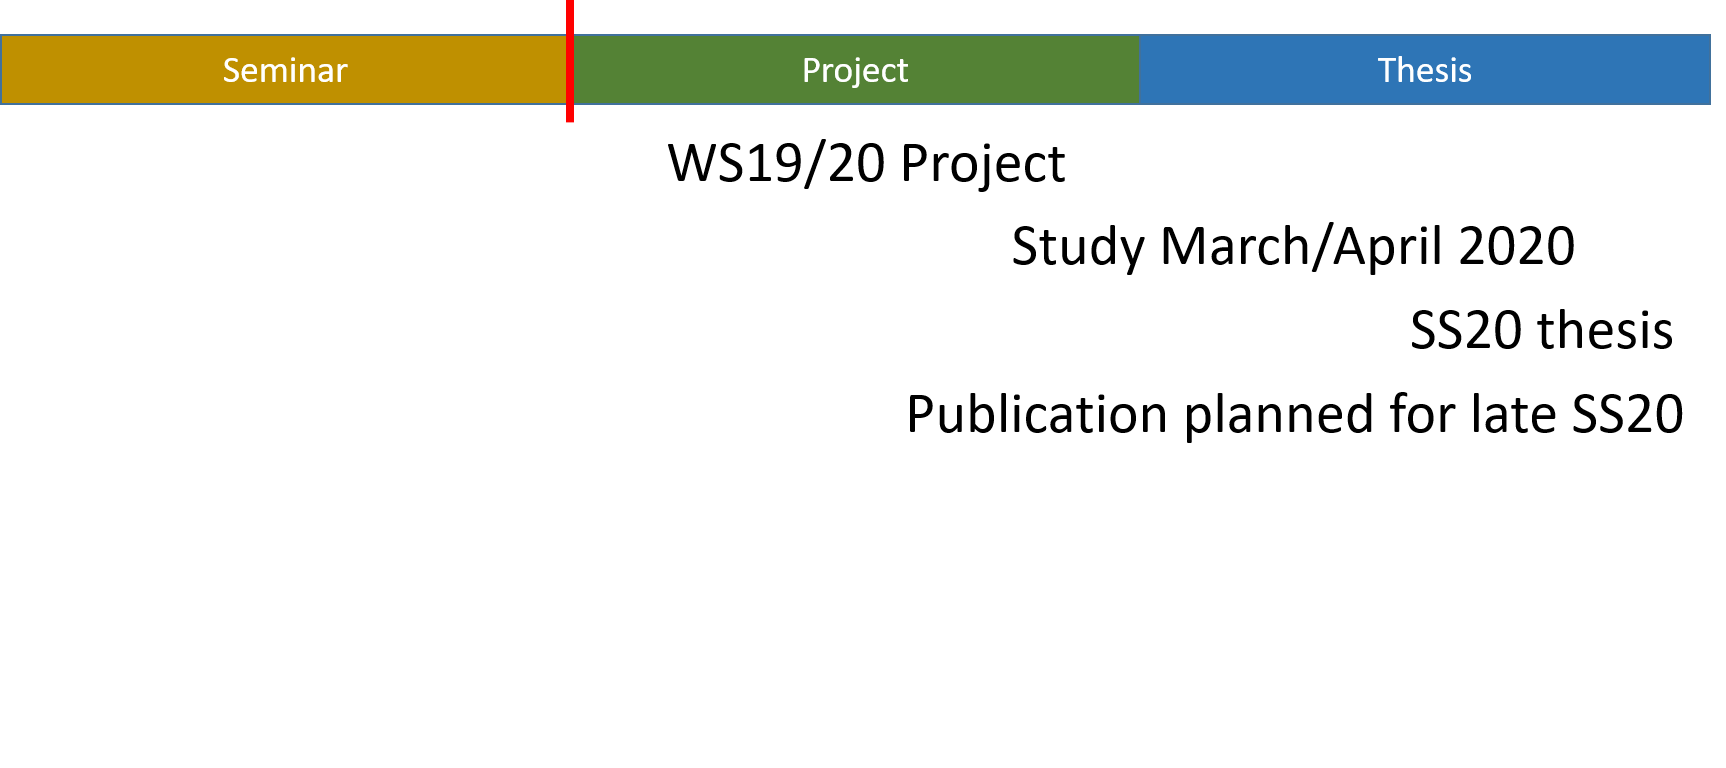
\includegraphics[width=1.0\textwidth]{img/outlook.png}
	\caption{Timetable for the master's thesis.}
	\label{fig:outlook}
\end{figure}

\begin{comment}
\section{Variables}
\subsection{Independent Variables}
\begin{itemize}
\item ego-centric
\item exo-centric
\item combined
\begin{itemize}
\item \textcolor{red}{variation of combined:} sequetial - parallel
\end{itemize}
\end{itemize}
further variations that could be interesting:
\begin{itemize}
\item body parts
\item sitting/standing
\item visual representation
\item degree of realism of avatar
\item guidance techniques: stopping at keyframes vs. fluent instructions
\item audio queues
\item feedback
\item fixed position of teacher and avatar, vs walking around
\end{itemize}
\subsection{Dependent variables}
Score. Combination of objective and subjective measurements.
\begin{itemize}
\item precision
\item subjective opinion of participant
\item stress level (EKG, HRV)
\item cognitive load
\item retention
\item reaction time
\end{itemize}
\section{Task}
\begin{itemize}
\item Tai Chi form, split in subtasks
\item Dance moves from single dance
\end{itemize}
variations:
\begin{itemize}
\item difficulty
\item complexity
\item abstract vs. real world
\item operate a control panel
\item escape the room
\item game    
\end{itemize}

\section{Hypothesis}
%hier wird ein mögliches studiendesign vorgestellt

\subsection{Aim of the Study}
The aim of the study is to investigate the influence of egocentric and exocentric perspectives on a virtual avatar during motor learning tasks.

\subsection{process}
There are two groups: one learn only with the egocentric perspective, the other one with the exocentric perspective on the virtual avatar.\\
To derive conclusions on body regions, every participant learns movements for three different body parts. The body parts are:
\begin{itemize}
\item \UB (UB)
\item \LB (LB)
\item \FB (FB)
\end{itemize}
To derive conclusion on movement types, two different movements per body part is learned. The two movement types are:
\begin{itemize}
\item mirrored movements
\item independent movements
\end{itemize}

\begin{center}
\begin{tabular}{ | c | c | c | c | }
\hline
& UB & LB & FB \\ \hline 
Ego & \parbox{4cm}{1 mirrored and 1 asynchronous movement} & \parbox{4cm}{1 mirrored and 1 independent movement} & \parbox{4cm}{1 mirrored and 1 independent movement} \\ \hline 
Exo & \parbox{4cm}{1 mirrored and 1 independent movement} & \parbox{4cm}{1 mirrored and 1 independent movement} & \parbox{4cm}{1 mirrored and 1 independent movement} \\ \hline
Ego/Exo & \parbox{4cm}{1 mirrored and 1 independent movement} & \parbox{4cm}{1 mirrored and 1 independent movement} & \parbox{4cm}{1 mirrored and 1 independent movement} \\
\hline
\end{tabular}
\label{table:studyDesign}
\end{center}

\subsection{Independent variables}
\begin{itemize}
\item perspective on the avatar (Ego/Exo centric)
\item body parts (\UB, \LB, \FB)
\item movement types (mirrored/independent movements)
\end{itemize}

\subsection{measures}
TBA
\end{comment}
	\chapter{Outlook}
\begin{itemize}
	\item timetable, what to do
\end{itemize}
	\bibliography{bib/lit}
	\bibliographystyle{plain}
	%\chapter{Scope}
\section{Motor Learning}
%beschreibung welche auf welche art von bewegungen sich hier beschränkt wird.
\begin{itemize}
	\item discrete movements
	\item closed skills
	\item at least 2 different movement categories
	\item how to measure movements
	\item posture vs movement
\end{itemize}

\section{Mixed Reality}
%begründen welchen auf welchen part des kontinuums man sich beschränkt
\begin{itemize}
	\item Milgram
	\item AR or VR
\end{itemize}

\section{Perspective}
%welche prespectiven behandelt werden und welche nicht


\section{Misc}
%welche einschränkungen gibt es noch. zb. das es kein feedback gibt, der realitätsgrad der avatare nicht evaluiert werden soll. erst zum schluss
\begin{itemize}
	\item synchron asynchron
	\item colocated/remote
	\item perspective
	\item hardware?
	\item feedback!
	\item real world, not abstract avatars
	\item only visuals - no audio or textual explanation
\end{itemize}
	%\chapter{Theory}
\section{Metholodgy}
sth like UX live cycle or participatory design
\section{HCI Theory}
sth like embodied cognition
Groundwork for designing VR motor learning systems

	%\section{Motivation}
äöü
	%\section{them. verw. arbeiten}
requirements: variablen zu untersuchen
	%\section{conclusion}
	%\section{Motor Learning}
\begin{itemize}
	\item for simplifying discussion introducing classification of movements and motor tasks.
	\item 2 important classification schemes:
	\begin{itemize}
		\item based on particular movements made: discrete, continuous, serial
		\item based on perceptual attributes of the task: open/closed
	\end{itemize}
	\item \underline{discrete movements}
\end{itemize}

	%\section{Zusammenfassungen von gelesenen papern}
\end{document}